\documentclass[10pt,a4paper]{article}
\usepackage{titling}
\usepackage[margin=1 in]{geometry}
\usepackage{graphicx}
\usepackage{listings}
\usepackage[normalem]{ulem}
\graphicspath{{.}}
\newcommand{\subtitle}[1]{%
  \posttitle{%
    \par\end{center}
    \begin{center}\large#1\end{center}
    \vskip0.5em}%
}

\begin{document}

\title{\vspace{-3cm}Hot Protocol Version 2 (HotPv2)}
\subtitle{Hottentot RPC Framework}
\author{Kamran Amini}

\maketitle

\rule{15cm}{0.4pt}

\tableofcontents
\newpage

\section {Introduction}
This document talks about request and response structures and mechanisms in Hottentot RPC Framework. Purpose of this protocol is to convey Method Invocation request and response. Current protocol is serialization transparent and can convey a method call with arguments produced with different serialization algorithms. In this version, Hottentot's runtimes can only work with internal serialization mechanism.

\section {Glossary}
  \bigskip
  \textbf {SERIALIZATION} \\ \indent {A process in which an object turns into a byte array to be transferred using a channel.} \\\\
  \textbf {STRUCT} \\ \indent {A term used for encapsulation of fields related to a specific entity. It is a structure and it will be generated differently for each programming language.} \\\\
  \textbf {IDL (INTERFACE DEFINITION LANGUAGE)} \\ \indent {An IDL is a language transparent to all programming languages which Hottentot supports. IDL can be generated to any target languages supported by Hottentot RPC Framework.} \\\\
  \textbf {HOT FILE} \\ \indent {A file which contains IDL. Hot files usually end with \texttt{.hot} extension.} \\\\
  \textbf {GENERATOR} \\ \indent {A tool for generating stub and struct source codes for a target programming language. Currently, generators for C++ and Java languages are available.} \\\\
  \textbf {RUNTIME} \\ \indent {A library for a specific programming language which performs Service and Proxy operations. Currently, runtimes are only available for C++ and Java.} \\\\
  \textbf {ENDPOINT} \\ \indent {Endpoint is a combination of IP address and a port. One service object or many can be bound to an endpoint.} \\\\
  \textbf {CURRENT ENDPOINT} \\ \indent {When talking about a proxy, Current Endpoint is an endpoint which client has used for connecting to server-side.} \\\\
  \textbf {SERVICE} \\ \indent {Service is an object serving method invocation requests.} \\\\
  \textbf {PROXY} \\ \indent {Proxy is an object which produces method invocation and other types of requests and receives the response. A proxy object talks to an endpoint at first and its request will be delegated to a service object in case of method invocation requests.} \\\\
  \textbf {PROXY-SIDE} \\ \indent {A software or library which tries to interact with service-side objects like endpoints, services, etc.} \\\\
  \textbf {SERVICE-SIDE} \\ \indent {A software or library which serves proxy-side requests and generates suitable response.} \\\\

\section {Algorithms}

\subsection {Fast Hash Algorithm}
A fast hashing algorithm developed by Zilong Tan. It has 2 versions. One generated 32-bit has value for a given byte array and the other one generates a 64-bit hash value for the input. Hottentot uses fast hash algorithm for generating system independent identifiers (ids) for services and methods.

\section {Request}
Each request consists of 1 mandatory and 2 optional fields.
\begin{itemize}
  \item \textbf{Request Type}: This field is mandatory. Using this field determines type of request.
  \item \textbf{Payload}: This files is optional and carries all necessary data to perform the request operation.
  \item \textbf{Request Digital Signature} This fields is optional and carries a PKI compatible digital signature over Request Type and Payload.
\end{itemize} 
Please notice that, there is no checksum or error detection block involved in request structure. This means that we trust underlying network connection for handling communication errors. Also security concerns like impersonation, eavesdropping or on-wire injection will not be discussed here. There is a dedicated chapter for explaining security issues and detailed provided solutions. Below figure shows the request structure.

\begin{figure}[!ht]
  \caption{HotPv2 Request Structure}
  \centering
    \scalebox{2.1}{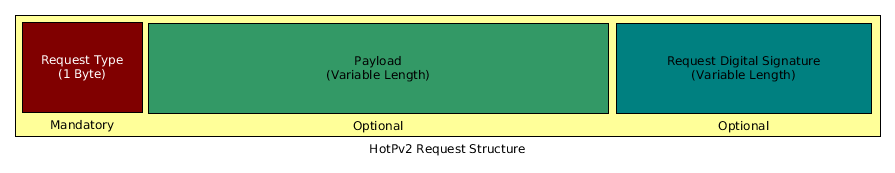
\includegraphics[width=0.5\textwidth]{hotpv2__request-type.png}}
\end{figure}

\subsection {Request Type}
Determines the request type and payload structure. Following C enumeration shows the possible values for this field.

\begin{verbatim}
enum RequestType { 
  Unknown = 0x00, 
  ServiceListQuery = 0x01, 
  MethodInvocation = 0x02,
  MethodListQuery = 0x03,
  ServiceInfoQuery = 0x04,
  MethodInfoQuery = 0x05,
  EndpointInfoQuery = 0x06,
  ProxyInfo = 0x07
};
\end{verbatim}

\noindent
Values can be:
\begin{itemize}
  \item \textbf{Unknown}: It means nothing to Hottentot service side and these requests should be ignored by implementation.
  \item \textbf{ServiceListQuery}: Proxy-side queries about the list of available services. Hottentot service runtime should return list of services exposed on current endpoint.
  \item \textbf{MethodInvocation}: Invokes a method on a specific service object.
  \item \textbf{MethodListQuery}: Proxy-side queries about the list of callable methods on a specific service object.
  \item \textbf{ServiceInfoQuery}: Proxy-side asks about parameters of a specific service.
  \item \textbf{MethodInfoQuery}: Proxy-side asks about parameters of a specific method.
  \item \textbf{EndpointInfoQuery}: Proxy-side asks about parameters of current endpoint.
  \item \textbf{ProxyInfo}: Proxy-side sends its parameters to current endpoint.
\end{itemize}

\subsection {Payloads}
Requests can have payloads. Many request types need data for their operations and payload carries the data. Following sections explain about payload structure for each request type. Please notice that, any needed piece of information or security object for authentication and authorization purposes will not be included in payloads and these objects will be transferred in \textit{Handshake} phase.

\subsubsection {Payload for \textit{Service List Query} Request Type}
A \textit{Service List Query} request has no payload. In other words, this request has only one byte carrying value 0x01 as \textit{Service List Query} request type identifier.

\begin{figure}[!ht]
  \caption{Structure of a Service List Query request.}
  \centering
    \scalebox{1.2}{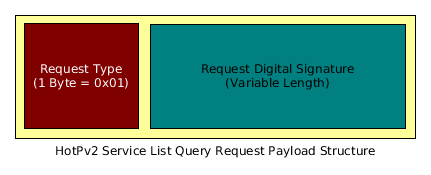
\includegraphics[width=0.5\textwidth]{hotpv2__service-list-query-request.png}}
\end{figure}

\subsubsection {Payload for \textit{Method Invocation} Request Type}
A \textit{Method Invocation} request payload consists of following fields:
\begin{itemize}
  \item Service Id (4 Bytes)
  \item Method Id (4 Bytes)
  \item Number of Arguments (1 Byte)
  \item Arguments as an array of LV Structures. (Variable Length)
\end{itemize}

\begin{figure}[!ht]
  \caption{HotPv2 Method Invocation Request Structure}
  \centering
    \scalebox{2.1}{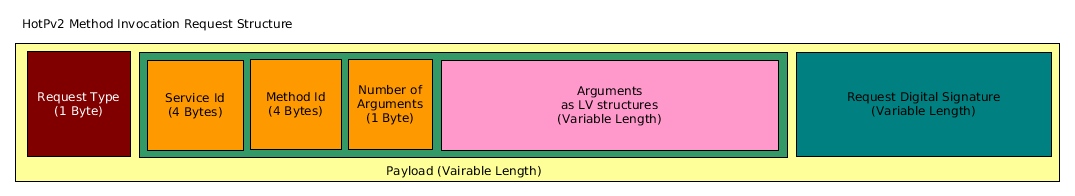
\includegraphics[width=0.5\textwidth]{hotpv2__method-invocation-request.png}}
\end{figure}

Figure 2 shows the structure of a request. Arguments can be transferred using LV structures. LV structures include Length and Value. Maximum length for a single LV structure is $2^{32} - 1$ since length values can be stored in a field at most 4 bytes. Figure 3 shows the LV structures in detail.

\begin{figure}[!ht]
  \caption{Structure of a Method Invocation request payload with arguments' LV structures.}
  \centering
    \scalebox{2.2}{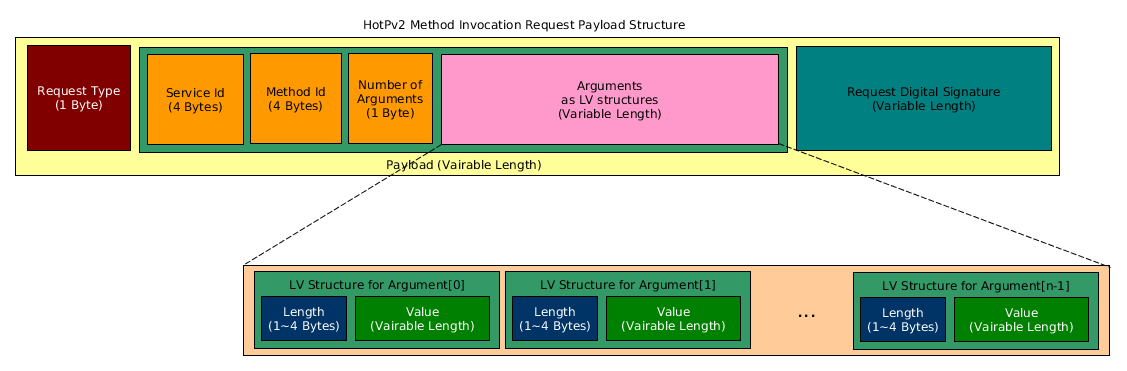
\includegraphics[width=0.5\textwidth]{hotpv2__method-invocation-request-payload-lv-structures.png}}
\end{figure}

Value can be any byte array but usually it is a serialized object. Serialization method can be anything. Hottentot itself provides an algorithm for serialization and \texttt {serialize()} and \texttt {deserialize()} methods are generated for every struct. Current stub generation mechanism works only with Hottentot's internal serialization.

\subsubsection {Payload for \textit{Method List Query} Request Type}
A \textit{Method List Query} request has following fields:
\begin{itemize}
  \item Service Id (4 Bytes)
\end{itemize}
This will return list of methods available on a service object identified by \textit{Service Id}.

\begin{figure}[!ht]
  \caption{Structure of a Method List Query request.}
  \centering
    \scalebox{1.5}{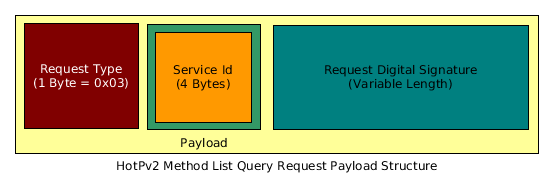
\includegraphics[width=0.5\textwidth]{hotpv2__method-list-query-request.png}}
\end{figure}

\subsubsection {Payload for \textit{Service Info Query} Request Type}
A \textit{Service Info Query} request has following fields:
\begin{itemize}
  \item Service Id (4 Bytes)
\end{itemize}
This will return the parameters and their values for a service object identified by \textit{Service Id}. Parameters and values are serialized according to LV structures. Structure for service parameters will be explained in future chapters.

\begin{figure}[!ht]
  \caption{Structure of a Service Info Query request.}
  \centering
    \scalebox{1.5}{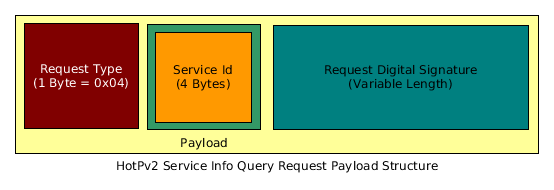
\includegraphics[width=0.5\textwidth]{hotpv2__service-info-query-request.png}}
\end{figure}

\subsubsection {Payload for \textit{Method Info Query} Request Type}
A \textit{Method Info Query} request has following fields:
\begin{itemize}
  \item Service Id (4 Bytes)
  \item Method Id (4 Bytes)
\end{itemize}
This will return the parameters and their values for a method identified by \textit{Method Id} on a specific service object identified by \textit{Service Id}. Parameters and values are serialized according to LV structures. Structure for method parameters will be explained in future chapters.

\begin{figure}[!ht]
  \caption{Structure of a Method Info Query request.}
  \centering
    \scalebox{1.5}{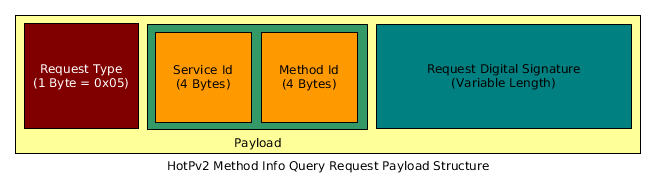
\includegraphics[width=0.5\textwidth]{hotpv2__method-info-query-request.png}}
\end{figure}

\subsubsection {Payload for \textit{Endpoint Info Query} Request Type}
A \textit{Endpoint Info Query} request has no fields, hence we have no payload. Parameters of current endpoint selected by proxy-side will be returned as response. Parameters are serialized according to LV structures.

\begin{figure}[!ht]
  \caption{Structure of a Endpoint Info Query request.}
  \centering
    \scalebox{1.2}{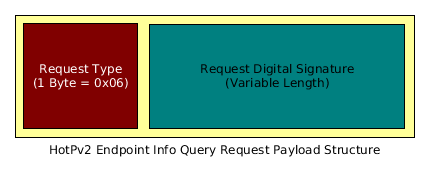
\includegraphics[width=0.5\textwidth]{hotpv2__endpoint-info-query-request.png}}
\end{figure}

\section {Future Features}
\begin{itemize}
  \item Version should be added to request and response structures.
\end{itemize}

\end{document}